%%%--------------------------------%%%
%%% UC8
%%%--------------------------------%%%

\newpage
% UC8 ====================================================
\subsubsection{Use Case Specification: \ac{UC}8 Risk Response Management}
\label{sec:domainBbi}
\begin{wrapfigure}{r}{0.3\textwidth}
	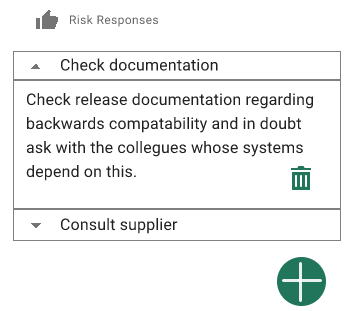
\includegraphics[width=0.3\textwidth]{Assets/UC_Screenshots/UC8S.png}
	\caption{Use Case 8: Mock Prototype}
	\label{fig:useCase8Detail}
\end{wrapfigure}

\paragraph*{Description}\mbox{}\\
Responses are ways to react to a risk. A new response can be added to a risk from the risk detail view. A response contains a name, a type and a description as well as the information whether the described steps have already been undertaken or not. Depending on the Type of risk a reminder is set to remind the risk owner to repeat the response tasks.\\
The risk owner can remove a response on a project risk if the project manager concurs.\\
If the risk is a pool risk the response can also be a pool response. Pool responses can only be removed if all project managers who currently reference the risk concur. However, pool responses can be deactivated for the current project with only the current project manager agreeing to prevent situationally unsuitable response reminders.\\
A new response to a pool risk can be turned into a pool response via a voting process among team members.
This is a CRUD use case.

\paragraph*{Basic Flow} \mbox{}\\
\noindent
Creating a response:
\begin{itemize}
	\vspace{-3mm}
	\setlength\itemsep{-1em}
	\item When the user clicks the "+" button at the risk detail view in the response section.
	\item Then the screen for adding a new response is opened.
	\item When the response form is filled by the user.
	\item And the user clicks on the "Add response" button.
	\item Then the risk is synced with the server.
\end{itemize}

\noindent
Reading a response:
\begin{itemize}
	\vspace{-3mm}
	\setlength\itemsep{-1em}
	\item The user is on the risk detail view for a project risk.
	\item By clicking on a response a detail view is expanded.
	\item For exiting the detail view a minimize button is clicked.
\end{itemize}

\noindent
Updating a response: 
\begin{itemize}
	\vspace{-3mm}
	\setlength\itemsep{-1em}
	\item The user is on the risk detail view for a project risk.
	\item In the risk response section there is a pen button, which opens an editing form.
	\item By clicking the "Save" button the risk owner is notified of the changes.
	\item If the owner concurs with the changes, they are synchronized with the server.
\end{itemize} 

\noindent
Deleting a response:
\begin{itemize}
	\vspace{-3mm}
	\setlength\itemsep{-1em}
	\item The user is on the risk detail site for a project risks.
	\item By clicking a "Delete" button the project manager receives a notification.
	\item If the project manager concurs, the response is deleted.
\end{itemize}

\paragraph*{Alternative Flows}\mbox{}\\
In addition to the CRUD functionalities responses attached to a risk that references a pool risk can be nominated for becoming a pool response and thus being attached to pool risk permanently. The voting process is the same as for pool risk nomination described in UC 5\ref{sec:domainBbf}.
The update and delete flows change if the response is a pool response attached to a pool risk.
\begin{itemize}
	\vspace{-3mm}
	\setlength\itemsep{-1em}
	\item Updating a pool response requires project manager concurrence.
	\item Deleting a pool response will trigger a voting process as described in UC 5\ref{sec:domainBbf}. However, it will be limited to project managers to prevent users from deleting unpleasant responses.
\end{itemize}


\paragraph*{Special Requirements and Preconditions}\mbox{}\\
The preconditions for this use case are:
\begin{enumerate}
	\vspace{-3mm}
	\setlength\itemsep{-1em}
	\item  A risk exists.
	\item The user is member of the project containing the risk.
	\item Deleting requires the user to also be the owner of the risk.
\end{enumerate}
For pool responses the following preconditions replace the above described:
\begin{enumerate}
	\vspace{-3mm}
	\setlength\itemsep{-1em}
	\item The response is attached to a pool risk.
\end{enumerate}

\paragraph*{Postconditions and Persistence}\mbox{}\\
Changes are directly reflected into the database via corresponding queries.

\subparagraph{Activity Diagram}\mbox{}\\
\begin{figure}[H]
	\centering
	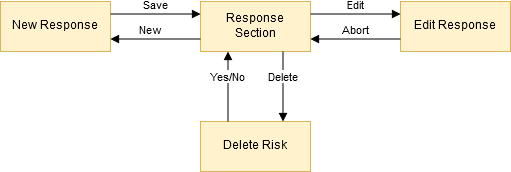
\includegraphics[width=0.8\textwidth]{Content/Domain/UC8RiskResponseCRUDactivitydiagram}
	\caption{Activity Diagram Use Case 8}
	\label{fig:label88}
\end{figure}

